\section{Results}\label{sec:results}
This sections presents the constraint on $\fnl$ from the DR9 LRG sample. The robustness of constraints are tested against various assumptions and details in survey mask, imaging weights, and calibration of data. The default analysis uses the covariance from $\fnl=0$ mocks. We also validate the modeling pipeline and characterize the amount of mitigation bias introduced in $\fnl$ after cleaning for systematics. 

\subsection{DR9 LRGs}

Fig. \ref{fig:cl_dr9} shows the measured power spectrum of the DESI imaging DR9 LRG sample with different imaging weights applied, the best fit theory predictions, and the mean and 1$\sigma$ error on angular power spectrum measured from the $\fnl=0$ lognormal simulations. Power spectra are similar with differences less than ??\% for small scales ($\ell > 2$), and as we go to larger scales, the differences become more significant. There is a little difference between linear cons II and linear all maps. This proves that our feature selection procedure has worked to identify the important maps. Comparing linear cons I to linear cons II, modes with $6\leq \ell < 10$ are different, indicating scales where psfsize-r is affecting the signal. Comparing nonlinear cons II to linear cons II, modes at the second bin ($4 \leq \ell < 6$) are very different, indicating the nonlinear approach is more flexible to reduce fluctuations on small scales as well large scales. 

\begin{figure}
    \centering
    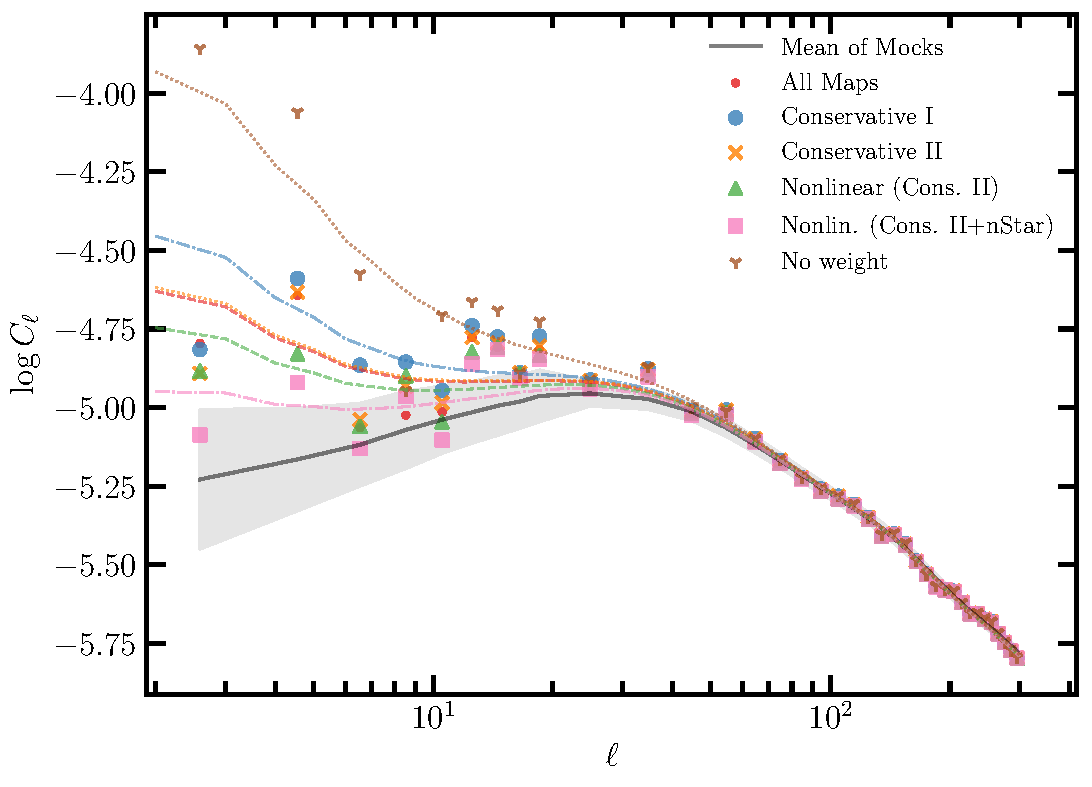
\includegraphics[width=0.45\textwidth]{figures/model_dr9.pdf} 
    \caption{Measured power spectrum of the DR9 LRG sample before and after correcting for systematics with their corresponding best fit theory predictions. The shade represents $1\sigma$ error constructed from the $\fnl=0$ mocks.}
    \label{fig:cl_dr9}
\end{figure}

\subsubsection{Calibrated constraints}

\begin{figure*}
    \centering
    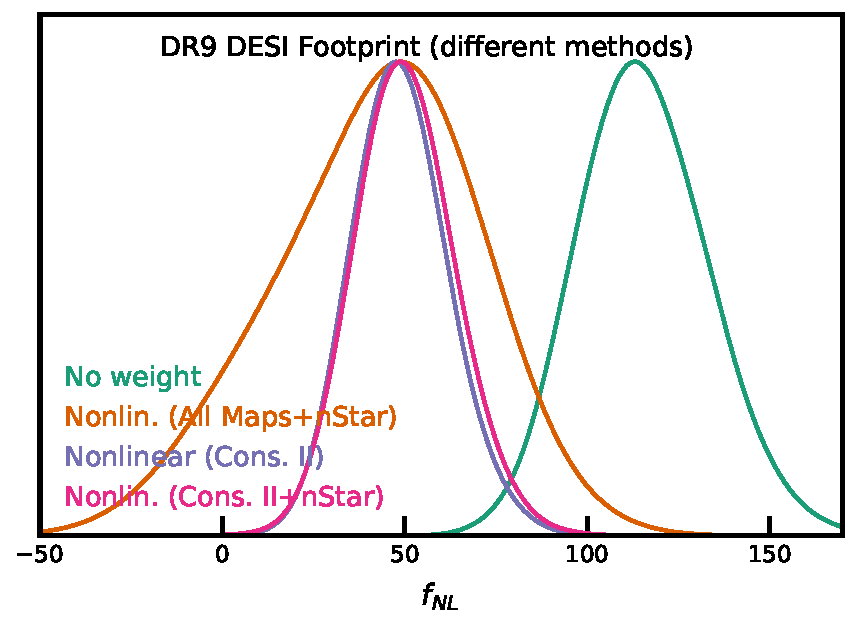
\includegraphics[width=0.45\textwidth]{mcmc_dr9methods1d.pdf}
    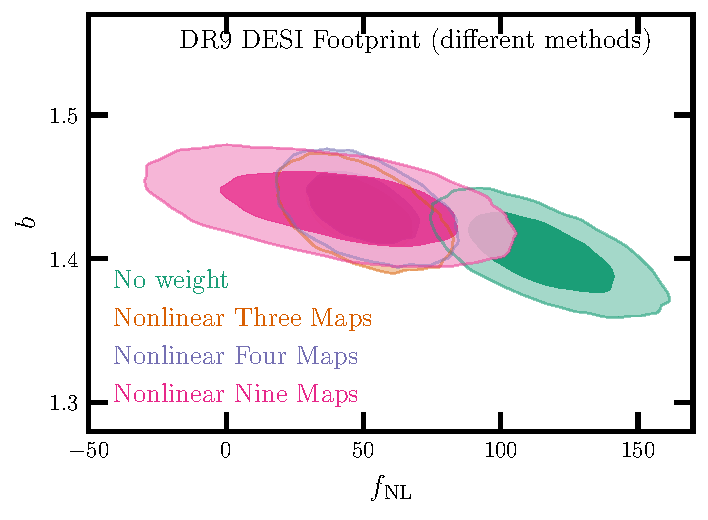
\includegraphics[width=0.45\textwidth]{figures/mcmc_dr9methods.pdf} 
    \caption{Calibrated 1D and 2D $\fnl$ constraints from the DR9 LRG sample before and after applying nonlinear cleaning methods. The dark and light 2D contours represent $68\%$ and $95\%$ confidence intervals, respectively.}\label{fig:mcmc_dr9}
\end{figure*}

\begin{table*}
    \caption{Calibrated best fit and marginalized mean estimates for $\fnl$ from fitting power spectrum of the DESI DR9 LRG sample before and after correcting for systematics. Degree of freedom is 34 (37 data points - 3 parameters).}
    \label{tab:dr9methodcalib}
   \centerline{%     
    \begin{tabular}{llllllll}
    \hline
    \hline
   &  & 	  & & $\fnl$ &  &  \\
   \cmidrule(r{.7cm}){3-6}
Footprint                               & Method & 	Best fit  & Mean & $ 68\%$ CL & $ 95\%$ CL & $\chi^{2}$ \\
    \hline
DESI                      & No Weight   & $113.18$& $115.49$& $ 98.14<\fnl<132.89$& $ 83.51<\fnl<151.59$ &   44.4\\
DESI                      & Nonlinear (Cons. II)& $ 47.38$& $ 48.81$& $ 36.08<\fnl< 61.44$& $ 25.03<\fnl< 75.64$ &   34.6\\
DESI                      & Nonlin. (Cons. II+nStar)& $ 48.92$& $ 50.10$& $ 36.88<\fnl< 63.31$& $ 24.87<\fnl< 77.78$ &   35.2\\
DESI                      & Nonlin. (All Maps+nStar)& $ 49.69$& $ 41.91$& $ 13.10<\fnl< 69.14$& $-15.96<\fnl< 91.84$ &   39.5\\
   \hline
    \end{tabular}
}
\end{table*}


Tab. \ref{tab:dr9methodcalib} summarizes the best fit and marginalized mean estimates of $\fnl$ from fitting power spectrum of the DR9 LRG sample using the nonlinear approach with various combinations of imaging templates. All constraints are accounted for the mitigation bias using the lognormal mocks, which is further discussed in \S \ref{ssec:contmocks}. With the corrections applied, we obtain $36.07 (25.03) < \fnl < 61.44(75.64)$ for nonlinear (conservative II), $36.88(24.87) < \fnl < 63.31(77.78)$ for nonlinear (conservative II + nStar), and $13.09(-15.95) < \fnl < 69.14(91.84)$ for nonlinear (all maps + nStar) at $68\% (95\%)$ confidence. Fig \ref{fig:mcmc_dr9} shows the 2D constraints with $68\%$ and $95\%$ confidence on $\fnl$ and $b$ for the DESI footprint from the DR9 sample before (no weight) and after applying different cleaning schemes. No weight constraint at $68\%$ is $98.14<\fnl<132.89$ with a best fit of $113.18$ and marginalized mean of $115.49$, and is more than $2\sigma$ off from zero. Applying imaging weights shifts constraints to lower $\fnl$ values, and $b$ is slightly pulled upward since excess clustering due to systematics is removed. Using all maps with the linear model does not change the results, showing that three maps are sufficient at the linear level to mitigate systematics.  As an alternative, using a nonlinear model with three maps shows around $1\sigma$ shift, with $68\%$ confidence at $18.91<\fnl<40.59$, inconsistent with zero for more than $2\sigma$. Adding a template for the local stellar density shift constraints by $1\sigma$, making it consistent with zero. As the most rigorous approach, using all maps and stellar density included results in more than $2\sigma$ shift. We emphasize that these shifts to lower $\fnl$ are somewhat expected as more input maps results in regressing more modes from cosmological clustering signal. Therefore, we use lognormal mocks to calibrate the amount of signal that is removed in each case and attempt to undo the effect.



\subsubsection{Robustness tests}

These results are subject to mitigation bias. $\fnl$ constraints from DR9 LRG sample is summarized in Table \ref{tab:dr9method}. First, we focus on the DESI footprint and then compare constraints obtained from each sub-survey. We also evaluate the robustness of constraints against various cuts and configurations. First, we compare how constraints from whole DESI footprint compares to those from each survey individually, namely BASS+MzLS, DECaLS Nouth, and DECaLS South. Fig. \ref{fig:mcmc_dr9reg} shows $68\%$ and $95\%$ confidence on $\fnl$ and $b$ from each individual survey or all combined as DESI. Constraints from all surveys are consistent and agree with each other within $68\%$. Both BASS+MzLS and DECaLS South are consistent with zero PNG, but DECaLS North deviates from zero at more than $2\sigma$. Adding the stellar density template does not change constraints from BASS+MzLS much, but it shifts DECaLS North and DECaLS South by $0.5\sigma$ and $\sigma$, respectively. This might indicate that there are some unresolved issues with stellar contamination in DECaLS North and DECaLS South. We note that differences are more significant when all maps and stellar density are used as input. This is expected as more maps mean the model has more freedom to take out clustering modes.


\begin{table*}
    \caption{Uncalibrated best fit and marginalized mean estimates for $\fnl$ from fitting power spectrum of DR9 LRGs before and after correcting for systematics. Degree of freedom is 34 (37 data points - 3 parameters).}
    \label{tab:dr9method}
   \centerline{%     
    \begin{tabular}{llllllll}
    \hline
    \hline
   &  & 	  & & $\fnl$ &  &  \\
   \cmidrule(r{.7cm}){3-6}
Footprint                               & Method & 	Best fit  & Mean & $ 68\%$ CL & $ 95\%$ CL & $\chi^{2}$ \\
    \hline
DESI                                    & No Weight   & $113.18$& $115.49$& $ 98.14<\fnl<132.89$& $ 83.51<\fnl<151.59$ &   44.4\\
DESI                                    & Linear (All Maps)& $ 36.05$& $ 37.72$& $ 26.13<\fnl< 49.21$& $ 16.31<\fnl< 62.31$ &   41.1\\
DESI                                    & Linear (Conservative I)& $ 49.58$& $ 51.30$& $ 38.21<\fnl< 64.33$& $ 27.41<\fnl< 78.91$ &   38.8\\
DESI                                    & Linear (Conservative II)& $ 36.63$& $ 38.11$& $ 26.32<\fnl< 49.86$& $ 16.36<\fnl< 63.12$ &   39.6\\
DESI                                    & Nonlinear (Cons. II)& $ 28.58$& $ 29.79$& $ 18.91<\fnl< 40.59$& $  9.47<\fnl< 52.73$ &   34.6\\
DESI                                    & Nonlin. (Cons. II+nStar)& $ 16.63$& $ 17.52$& $  7.51<\fnl< 27.53$& $ -1.59<\fnl< 38.49$ &   35.2\\
DESI                                    & Nonlin. (All Maps+nStar)& $ -5.87$& $ -9.19$& $-21.45<\fnl<  2.40$& $-33.81<\fnl< 12.06$ &   39.5\\
DESI (imag. cut)                  & Nonlin. (Cons. II)& $ 29.16$& $ 30.57$& $ 19.05<\fnl< 42.18$& $  9.01<\fnl< 54.81$ &   35.8\\
DESI (comp. cut)                 & Nonlin. (Cons. II)& $ 28.07$& $ 29.48$& $ 18.38<\fnl< 40.50$& $  8.81<\fnl< 53.10$ &   34.5\\
DESI                                    & Nonlin. (Cons. II)+$f_{\rm NL}=76.92$ Cov& $ 31.62$& $ 33.11$& $ 20.94<\fnl< 45.24$& $ 10.56<\fnl< 59.16$ &   33.5\\
\hline
BASS+MzLS                        & Nonlin. (Cons. II)& $ 15.43$& $ 19.01$& $ -1.17<\fnl< 39.43$& $-19.19<\fnl< 63.56$ &   35.6\\
BASS+MzLS                        & Nonlin. (Cons. II+nStar)& $ 13.12$& $ 15.39$& $ -4.59<\fnl< 35.56$& $-24.88<\fnl< 59.31$ &   34.7\\
BASS+MzLS                        & Nonlin. (All Maps+nStar)& $ -3.73$& $ -6.34$& $-27.11<\fnl< 13.75$& $-47.44<\fnl< 33.94$ &   36.8\\
BASS+MzLS (imag. cut)      & Nonlin. (Cons. II)& $ 25.03$& $ 29.12$& $  6.16<\fnl< 52.44$& $-14.22<\fnl< 80.54$ &   36.2\\
BASS+MzLS (comp. cut)     & Nonlin. (Cons. II)& $ 16.99$& $ 20.90$& $  0.26<\fnl< 41.76$& $-18.30<\fnl< 67.12$ &   35.8\\
DECaLS North                     & Nonlin. (Cons. II)& $ 41.02$& $ 44.89$& $ 23.33<\fnl< 66.78$& $  4.96<\fnl< 93.02$ &   41.1\\
DECaLS North                     & Nonlin. (Cons. II+CALIBZ+HI)& $ 55.46$& $ 60.44$& $ 36.78<\fnl< 84.05$& $ 17.86<\fnl<112.81$ &   38.4\\
DECaLS North                     & Nonlin. (Cons. II+nStar)& $ 31.45$& $ 34.78$& $ 14.14<\fnl< 55.79$& $ -5.81<\fnl< 80.80$ &   41.2\\
DECaLS North                     & Nonlin. (All Maps+nStar)& $  0.81$& $ -5.68$& $-29.73<\fnl< 16.71$& $-53.15<\fnl< 36.19$ &   45.1\\
DECaLS North + islands      & Nonlin. (Cons. II)& $ 41.05$& $ 44.82$& $ 23.58<\fnl< 66.08$& $  6.40<\fnl< 91.42$ &   40.7\\
DECaLS North (imag. cut)   & Nonlin. (Cons. II)& $ 43.27$& $ 48.39$& $ 24.60<\fnl< 72.50$& $  4.71<\fnl<101.42$ &   35.1\\
DECaLS North (comp. cut)  & Nonlin. (Cons. II)& $ 40.55$& $ 44.63$& $ 22.41<\fnl< 67.11$& $  3.95<\fnl< 94.06$ &   41.4\\
DECaLS South                    & Nonlin. (Cons. II)& $ 31.24$& $ 33.21$& $ 14.89<\fnl< 52.40$& $ -5.11<\fnl< 74.35$ &   30.2\\
DECaLS South                    & Nonlin. (Cons. II+CALIBZ+HI)& $ 33.79$& $ 37.50$& $ 17.71<\fnl< 57.42$& $ -0.31<\fnl< 80.94$ &   30.8\\
DECaLS South                    & Nonlin. (Cons. II+nStar)& $ 14.34$& $  6.28$& $-21.19<\fnl< 30.01$& $-53.63<\fnl< 49.51$ &   31.9\\
DECaLS South                    & Nonlin. (All Maps+nStar)& $-36.76$& $-32.01$& $-49.38<\fnl<-13.61$& $-65.26<\fnl<  7.52$ &   31.5\\
DECaLS South + DEC < $-30$ & Nonlin. (Cons. II)& $ 43.79$& $ 46.79$& $ 30.16<\fnl< 63.41$& $ 16.38<\fnl< 82.72$ &   23.8\\
DECaLS South (imag. cut)        & Nonlin. (Cons. II)& $ 26.47$& $ 23.36$& $  3.18<\fnl< 47.84$& $-57.69<\fnl< 71.39$ &   30.0\\
DECaLS South (comp. cut)       & Nonlin. (Cons. II)& $ 29.62$& $ 31.76$& $ 13.00<\fnl< 51.58$& $ -9.78<\fnl< 74.28$ &   29.7\\
   \hline
    \end{tabular}
}
\end{table*}


\begin{itemize}
\item \textbf{Pixel completeness}
We remove pixels with low completeness from the DESI footprint by applying $f_{\rm pix}>0.5$, and find that the impact is negligible. Specifically, the cut removes \mr{$.6\%$} survey area and causes best fit $\fnl$ shifts only around $2\%$, from 28.58 to 28.07, see \textit{comp cut} Table \ref{tab:dr9method}. When investigated this impact on each region separately, BASS+MzLS increases around $10\%$, DECaLS North decreases $1\%$, and DECaLS South decreases around $5\%$.

\item \textbf{Imaging quality}
We remove pixels with poor imaging from the DESI footprint by applying the following cuts on imaging properties; $E[B-V]<0.1$, $nStar < 3000$, $depth_{g} > 23.2$, $depth_{r} > 22.6$, $depth_{z} > 22.5$, $psfsize_{g}<2.5$, $psfsize_{r}<2.5$, and $psfsize_{z}<2$. Overall the constraints are consistent despite best fit and marginalized mean estimates shift. Quantitatively, we lose about $8.2\%$ survey area, and the best fit $\fnl$ estimate changes about $2\%$ from $28.58$ to $29.16$. See \textit{imag cut} in Table \ref{tab:dr9method}. For BASS+MzLS only, the imaging cut increases the best fit by $62\%$ from $15.43$ to $25.03$. For DECaLS North and DECaLS South, the best fit increases by $5\%$ and $15\%$ respectively.

\item \textbf{Covariance}
We now use the mocks with $\fnl=76.92$ to construct a covariance matrix, and with the new covariance we observe a $12\%$ increase in the $\fnl$ constraint uncertainties and $11\%$ increase in the best fit estimate of $\fnl$.

\item \textbf{Lowest $\ell$} 
We decrease the largest mode (or increase the lowest $\ell$) used in estimating the best fit and $68\%$ confidence intervals. Fig. \ref{fig:mcmc_dr9elmin} illustrates the results for the DESI footprint and how they compared to BASS+MzLS, DECaLS North, or DECaLS South only results. Points represent marginalized mean estimates of $\fnl$ and errorbars represent $68$\% confidence from MCMC results.Overall we find that the constraints are robust against the largest mode.

\item \textbf{External maps} We also derive imaging weights using additional external maps for the neutral hydrogen column density (HI) and magnitude calibration errors in the z band (CALIBZ). With the new weights, we find the best fit estimates increase from $41.02$ to $55.46$ for DECaLS North and from $31.24$ to $33.79$ for DECaLS South.

\item \textbf{Declination cut} Our default analysis do not use the spurious islands in DECaLS North and DECaLS South below DEC = -30 to avoid potential calibration issues. \mr{PANASTARS are used for calibration below DEC of -30.} Without these cuts, best fit $\fnl$ estimates increase from $31.24$ to $43.79$ for DECaLS South and decrease from $41.02$ to $41.05$. This indicates that indeed there is an issue with DECaLS South below DEC of $-30$.

\end{itemize}

Overall we find that the declination cut is necessary for DECaLS South, while adding external templates for HI and CALIBZ, using a different covariance, or applying imaging and completeness cuts do not alter the constraints significantly.


\begin{figure}
    \centering
    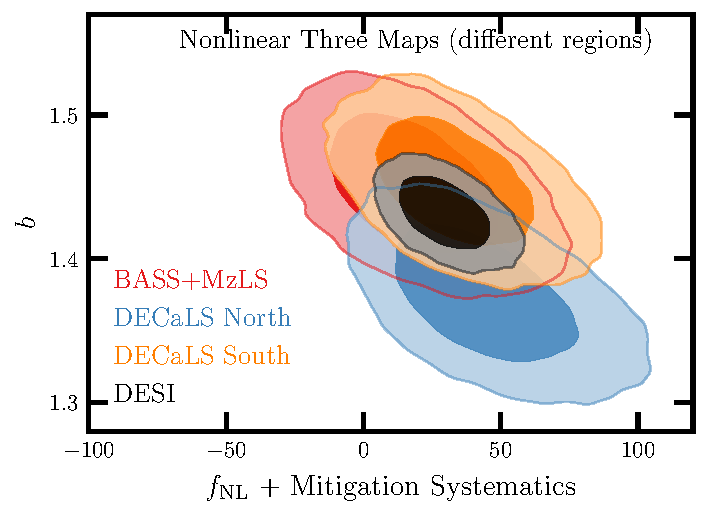
\includegraphics[width=0.45\textwidth]{figures/mcmc_dr9regions.pdf} 
    \caption{Uncalibrated 2D constraints from the DR9 LRG sample for each imaging survey compared with that for the whole DESI footprint. The dark and light shades represent the $68\%$ and $95\%$ confidence intervals, respectively.}\label{fig:mcmc_dr9reg}
\end{figure}




\begin{figure}
    \centering
    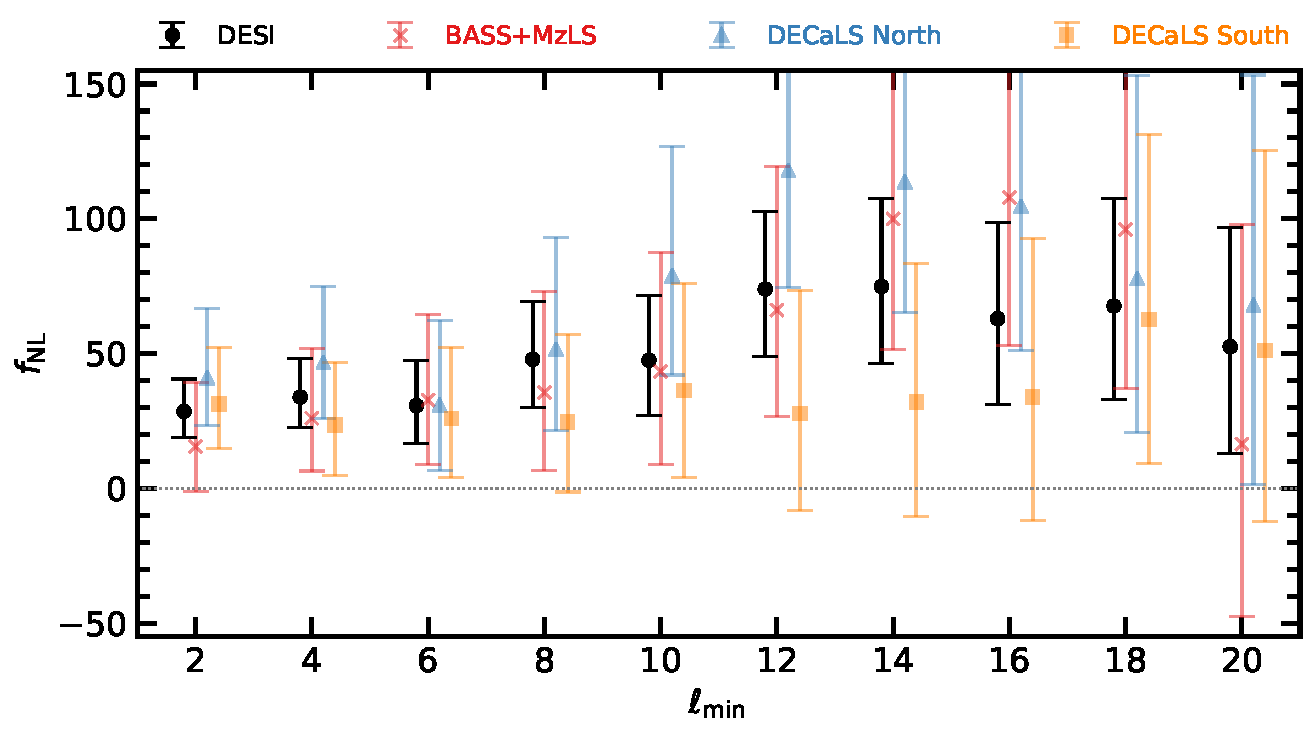
\includegraphics[width=0.45\textwidth]{figures/fnl_elmin.pdf}     
    \caption{Robustness of the uncalibrated DR9 constraints w.r.t. the largest scale (lowest $\ell$ mode) used in MCMC regression. Points represent marginalized mean estimates of $\fnl$ and errorbars represent $68$\% confidence.}\label{fig:mcmc_dr9elmin}
\end{figure}



\subsection{Lognormal Mocks}

\subsubsection{Clean mocks}
Corner plots of the PNG parameter $\fnl$ and bias coefficient are shown in Fig. \ref{fig:mcmc_mocks} for fitting the mean power spectrum of mocks, with and without $\fnl$. Best fit estimates, marginalized mean, $1\sigma$ and $2\sigma$ confidence intervals are summarized in Tab. \ref{tab:mocksmcmc}. Fig \ref{fig:mcmc_mocks} (right) shows confidence contours for different combinations of target variable (e.g., either power spectrum or its log transform) and covariance matrix. First we attempt to understand the impact of covariance on confidence intervals. We fit the mean power spectrum of $\fnl=76.9$ mocks or its log transformation using covariance matrices constructed from the same set of mocks or from the $\fnl=0$ mocks. When covariance is consistent with mean, the difference between fitting power spectrum and log of it is only 2\%. If a wrong covariance is used for the log power, the effect is only $7\%$. However, when mean power spectrum of the $\fnl=76.9$ mocks is fit using the covariance matrix estimated from the $\fnl=0$ mocks, the constraints improve by a factor of $5$, simply due to a false higher signal to noise ratio. Therefore, we argue that fitting logarithm of power spectrum would remove the need for having $\fnl$-dependent covariance matrices and make the constraints less sensitive to covariance construction. Fig. \ref{fig:mcmc_mocks} (left) shows the confidence contours for $\fnl=0$ mocks when fit is done to the log of mean spectra of $\fnl=0$ mocks for the different regions. We find that the underlying true $\fnl$ value is recovered within $2\sigma$ confidence. \mr{Add a paragraph for the constraining power vs fsky}.

Fig \ref{fig:bestfit_mocks} shows the best fit estimates for $b$ vs $\fnl$ for $\fnl=0$ and $=76.92$ mocks in the left and right, respectively. Truth values are represented via the dotted lines. The points are color-coded with the minimum $\chi^{2}$ from fit for each realization. The histograms of best fit $\fnl$ estimates are plotted in the background. We obtain $\fnl=MU\pm STD$ and $=MU\pm STD$ for the left and right panels, respectively.

\begin{table*}
  %\begin{center}
    \caption{Best fit and marginalized mean estimates for $\fnl$ from fitting the mean power spectrum of the mocks. Degree of freedom is 34 (37 data points - 3 parameters).}   
    \label{tab:mocksmcmc}  
   \centerline{%
    \begin{tabular}{llllllll}
    \hline
    \hline
   &  & & & & $\fnl$ &  \\
   \cmidrule(r{.7cm}){4-7}    
Mock / $\fnl$ &  Footprint   &  Observable & 	Best fit  & Mean & $ 68\%$ CL & $ 95\%$ CL & $\chi^{2}$ \\
    \hline
Clean $76.92$ & DESI & log$C_{\ell}$           & $ 77.67$& $ 77.67$& $ 77.17<\fnl< 78.16$& $ 76.71<\fnl< 78.64$ &   38.8\\
Clean $76.92$ & DESI & $C_{\ell}$              & $ 77.67$& $ 77.65$& $ 77.17<\fnl< 78.14$& $ 76.70<\fnl< 78.60$ &   39.0\\
Clean $76.92$ & DESI & log$C_{\ell}$ + $f_{\rm NL}=0$ cov & $ 77.70$& $ 77.71$& $ 77.25<\fnl< 78.17$& $ 76.81<\fnl< 78.63$ &   39.9\\
Clean $76.92$ & DESI & $C_{\ell}$ + $f_{\rm NL}=0$ cov & $ 77.03$& $ 77.02$& $ 76.93<\fnl< 77.12$& $ 76.83<\fnl< 77.22$ &  207.6\\
\hline
Clean $0$ & DESI         &  log$C_{\ell}$     & $  0.36$& $  0.36$& $  0.06<\fnl<  0.65$& $ -0.23<\fnl<  0.94$ &   35.7\\
Clean $0$ & DECaLS North &  log$C_{\ell}$     & $  0.07$& $  0.06$& $ -0.47<\fnl<  0.60$& $ -1.00<\fnl<  1.12$ &   26.7\\
Clean $0$ & DECaLS South &  log$C_{\ell}$     & $  0.67$& $  0.67$& $  0.13<\fnl<  1.22$& $ -0.40<\fnl<  1.75$ &   34.3\\
Clean $0$ & BASS+MzLS    &  log$C_{\ell}$     & $  0.83$& $  0.82$& $  0.25<\fnl<  1.40$& $ -0.31<\fnl<  1.96$ &   39.4\\
\hline
    \end{tabular}
    }
\end{table*}


\begin{figure}
    \centering
    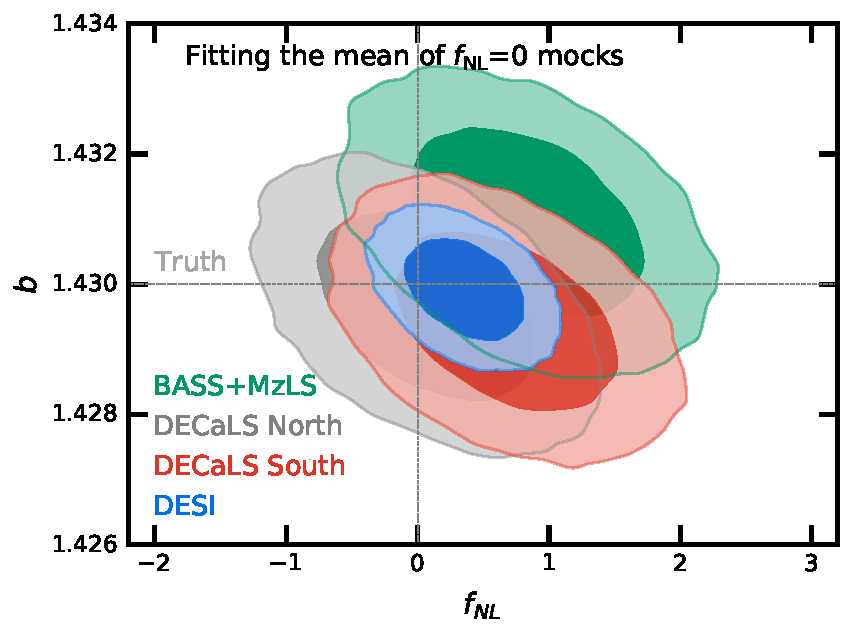
\includegraphics[width=0.45\textwidth]{figures/mcmc_zero.pdf} 
    \caption{68\% and 95\% confidence contours from the mean power spectrum of the $\fnl=0$ mocks for the DESI footprint and sub-imaging surveys. The truth values are represented by vertical and horizontal lines.}\label{fig:mcmc_mocks0}
\end{figure}

\begin{figure}
    \centering
    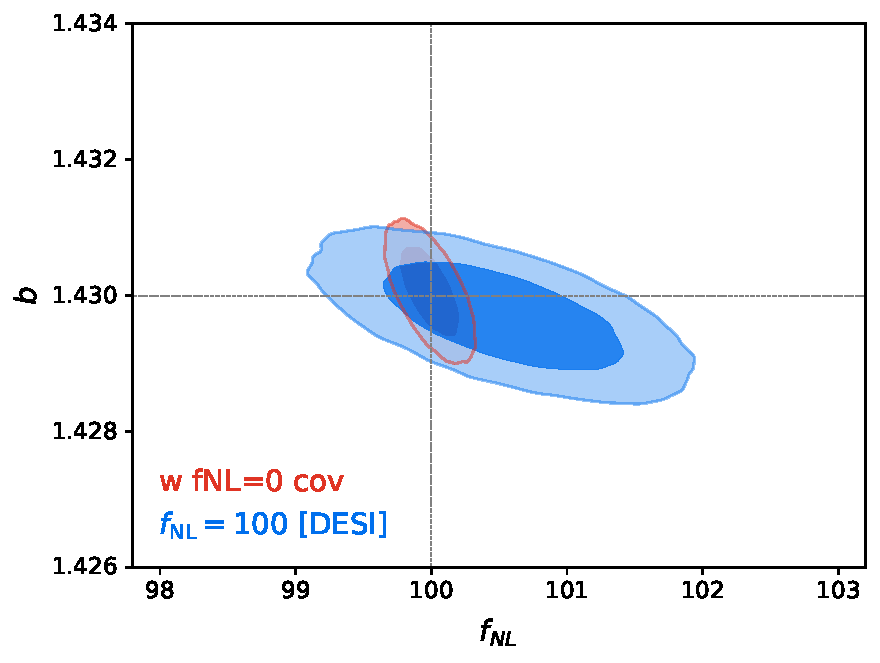
\includegraphics[width=0.45\textwidth]{figures/mcmc_po100.pdf} 
    \caption{68\% and 95\% confidence contours of fitting the mean power spectrum or its log transformation from the $\fnl=76.92$ mocks for the DESI footprint. Using the $\log C_{\ell}$ fitting yield constraints that are insensitive to the covariance used. The truth values are represented by vertical and horizontal lines.}\label{fig:mcmc_mocks100}
\end{figure}

\begin{figure}
    \centering
    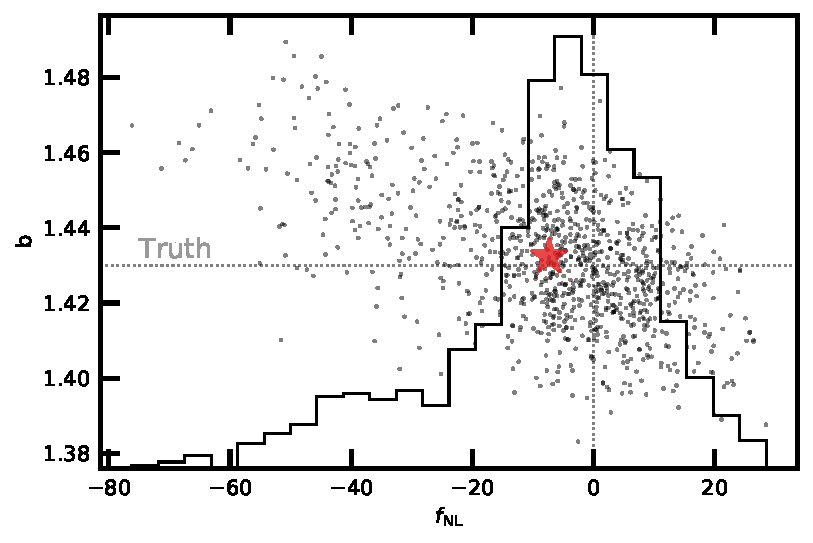
\includegraphics[width=0.45\textwidth]{figures/bestfit_zero.pdf} 
    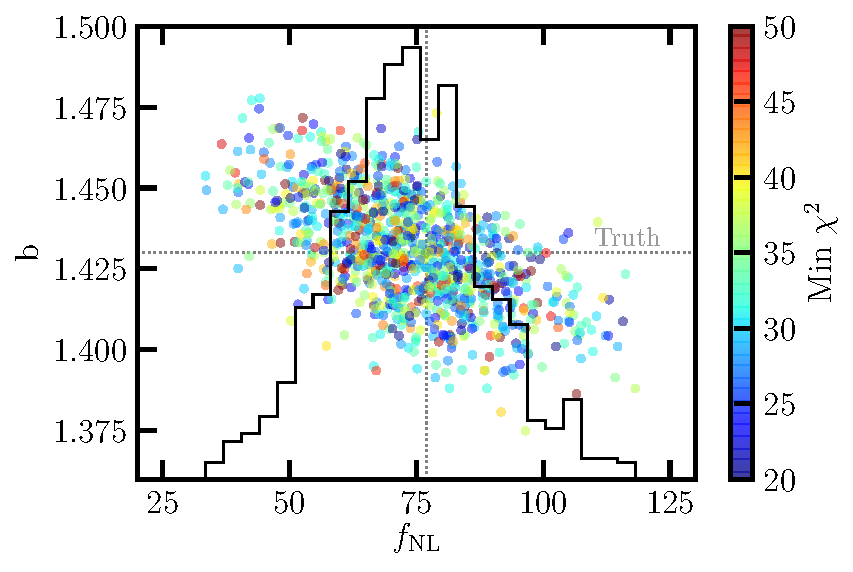
\includegraphics[width=0.45\textwidth]{figures/bestfit_po100.pdf}         
    \caption{Top: 68\% and 95\% confidence contours for $\fnl=0$ (left) and $76.92$ (right) mocks. Using the $\log C_{\ell}$ fitting yield constraints that are insensitive to the covariance used. Bottom: best fit estimates from fitting 1000 lognormal mocks with $\fnl=0$ (left) and $76.92$ (right) in the DESI footprint. The truth values are represented by vertical and horizontal lines.}\label{fig:bestfit_mocks}
\end{figure}




\subsubsection{Contaminated mocks}\label{ssec:contmocks}
\begin{table*}
  %\begin{center}
    \caption{Best fit and marginalized estimates for $\fnl$ from fitting the mean power spectrum of the mocks before and after applying imaging weights. }   
    \label{tab:contmocksmcmc}  
   \centerline{%
    \begin{tabular}{lllllll}
    \hline
    \hline
   &  & 	  & & & $\fnl$ &  \\
   \cmidrule(r{.7cm}){3-6}    
Mock / $\fnl$ & Method & Best fit  & Mean & $ 68\%$ CL & $ 95\%$ CL & $\chi^{2}$ \\
    \hline
Clean $0$ & No Weight                         & $  0.36$& $  0.36$& $  0.06<\fnl<  0.65$& $ -0.23<\fnl<  0.94$ &   35.7\\
Clean $0$ & ConsII                            & $-11.64$& $-11.65$& $-12.00<\fnl<-11.30$& $-12.34<\fnl<-10.97$ &   86.8\\
Clean $0$ & ConsII+nStar                      & $-20.14$& $-20.13$& $-20.44<\fnl<-19.82$& $-20.74<\fnl<-19.52$ &  472.8\\
Clean $0$ & All Maps+nStar                    & $-26.91$& $-26.92$& $-27.16<\fnl<-26.68$& $-27.39<\fnl<-26.46$ & 5481.0\\
Contaminated $0$ & ConsII                       & $-12.12$& $-12.13$& $-12.48<\fnl<-11.78$& $-12.83<\fnl<-11.44$ &   94.0\\
Contaminated $0$ & ConsII+nStar                 & $-20.97$& $-20.98$& $-21.28<\fnl<-20.67$& $-21.58<\fnl<-20.37$ &  556.3\\
Contaminated $0$ & All Maps+nStar               & $-28.13$& $-28.13$& $-28.36<\fnl<-27.90$& $-28.59<\fnl<-27.67$ & 6760.5\\
\hline
Clean $76.92$ & No Weight                       & $ 77.67$& $ 77.67$& $ 77.17<\fnl< 78.16$& $ 76.71<\fnl< 78.64$ &   38.8\\
Clean $76.92$ & ConsII                              & $ 54.57$& $ 54.57$& $ 54.14<\fnl< 55.01$& $ 53.72<\fnl< 55.45$ &  603.5\\
Clean $76.92$ & ConsII+nStar                     & $ 38.38$& $ 38.38$& $ 37.99<\fnl< 38.78$& $ 37.60<\fnl< 39.16$ &  537.0\\
Clean $76.92$ & All Maps+nStar                  & $  6.04$& $  6.04$& $  5.72<\fnl<  6.36$& $  5.41<\fnl<  6.67$ &  694.0\\
Contaminated $76.92$ & ConsII                   & $ 54.01$& $ 54.00$& $ 53.57<\fnl< 54.44$& $ 53.15<\fnl< 54.86$ &  588.0\\
Contaminated $76.92$ & ConsII+nStar             & $ 37.48$& $ 37.49$& $ 37.09<\fnl< 37.88$& $ 36.70<\fnl< 38.27$ &  510.7\\
Contaminated $76.92$ & All Maps+nStar           & $  4.59$& $  4.58$& $  4.26<\fnl<  4.90$& $  3.95<\fnl<  5.22$ &  649.7\\
\hline
    \end{tabular}
    }
\end{table*}


With template based mitigation, the measured power spectrum is biased and the amount of bias depends on the number of input templates. We use a linear model with the set of conservative II maps to simulate imaging systematics in our lognormal density fields. Then, we apply the cleaning method based on nonlinear model with Conservative II, Conservative II + nStar, or All Maps + nStar sets of imaging maps to both set of mocks; with or without systematic effects (dashed or soild), and with and without $\fnl$. The marginalized mean, confidence intervals, and best fit estimates are presented in Tab \ref{tab:contmocksmcmc}. This test indicates that as more maps are input to the nonlinear model, more power is removed, and thus the constraints are systematically shifted to lower $\fnl$ values. Fig \ref{fig:fnlbias} shows the true $\fnl$ value and the measured $\fnl$ value from fitting the mean of mocks. The results for the contaminated mocks before cleaning (No weight) is not shown for clarity. From this graph, then a pair of linear coefficients are to be found for mapping measured $\fnl$ to true $\fnl$ values. At the first iteration, we think these coefficients should be applied to the values presented in Tab \ref{tab:dr9method}.


\begin{figure}
\centering
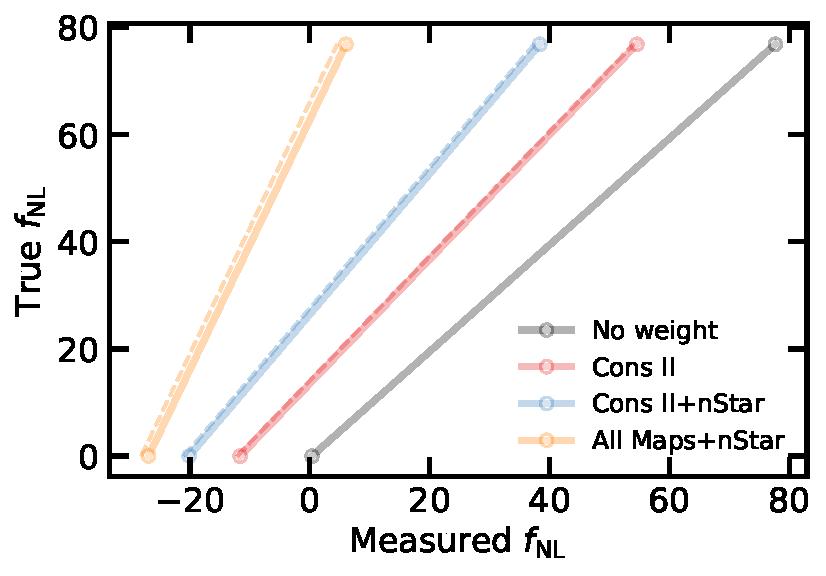
\includegraphics[width=0.45\textwidth]{figures/fnlbias}
\caption{True $\fnl$ vs measured $\fnl$ from the mean of the mocks with (dashed) and without systematics (solid).}\label{fig:fnlbias}
\end{figure}